\begin{frame}{Το έργο RELIEF: η λύση}


\noindent\makebox[\linewidth][c]{%
\begin{minipage}{\linewidth}
  \begin{minipage}{0.5\linewidth}
    \begin{figure}
      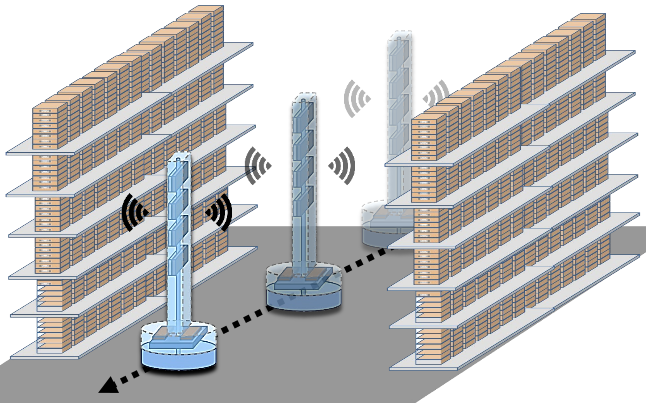
\includegraphics[height=101pt,width=180pt]{./figures/slides/01/relief_concept.png}
      %\caption{}
    \end{figure}
  \end{minipage}
  \hfill
 \begin{minipage}{0.5\linewidth}
 \begin{enumerate}
   \item Τοποθέτηση RFID ετικετών σε προϊόντα
   \item Αυτόνομα επίγεια οχήματα με RFID αναγνώστες
 \end{enumerate}
  \end{minipage}
\end{minipage}
}

\note{\footnotesize
Το έργο RELIEF στο οποίο εργάσθηκα εδώ στο πανεπιστήμιο είχε ως στόχο την
κατασκευή μίας σειράς από \textbf{αυτόνομα} ρομπότ τα οποία είναι ικανά να
καταγράφουν το απόθεμα μίας αποθήκης και να εκτιμούν τη θέση των εμπορευμάτων
μέσω τεχνολογίας RFID, ώστε αυτές οι ενέργειες να γίνονται ακόμα και σε
καθημερινή βάση, με ελάχιστη εμπλοκή ανθρώπων. Η πρώτη λοιπόν απαίτηση που
τέθηκε για τα επίγεια ρομπότ του έργου ήταν να είναι ικανά να πλοηγούνται
αυτόνομα στο χώρο.
%Σε πραγματικές συνθήκες μπορείτε να φανταστείτε πως προτού
%κλείσει η αποθήκη το βράδυ, ή ακόμα και κατά τη διάρκεια μίας εργάσιμης
%μέρας, στο ρομπότ δίνεται η εντολή να περάσει από συγκεκριμένες περιοχές του
%χώρου ώστε να σαρώσει όλα τα ράφια στα οποία υπάρχουν αντικείμενα.
Η αυτονομία της πλοήγησης είναι κρίσιμη γιατί αφαιρεί την απαίτηση για ακριβό
εξωτερικό εξοπλισμό πάνω στον οποίο θα μπορούσε να οδηγείται το ρομπότ, ενώ
ταυτόχρονα το κάνει εν δυνάμει ικανό να μπορεί να εκτελεί τις ενέργειές του
απρόσκοπτα ενώ υπάρχουν γύρω του κινούμενα εμπόδια όπως ανθρώποι ή μηχανήματα.}

\end{frame}
